 
\documentclass[12pt, a4paper]{article}
\usepackage{graphicx}
\usepackage{mathtools}
\usepackage{xcolor}
\usepackage{amsmath}
\usepackage{caption}
\usepackage[italian]{babel}
\usepackage{eso-pic}
\usepackage{setspace}
\usepackage{multirow}
\usepackage{array}
\usepackage{geometry}
\usepackage{longtable}
\graphicspath{ {./immagini/} }
\linespread{1.1}
\binoppenalty=10000 %impedisce di separare a capo formule matematiche nel testo
\relpenalty=10000
\geometry{
 total={170mm,257mm},
 left=20mm,
 top=15mm,
 bottom=28mm
 }
\title{\textbf{\scalebox{1.4}{\text{{\Huge Pendolo}}}}}
\date{}

\begin{document}
\maketitle
\AddToShipoutPictureBG*{%
  \AtPageUpperLeft{%
    \hspace{\paperwidth}%
    \raisebox{-\baselineskip}{%
      \makebox[0pt][r]{\textbf{Gruppo 10}: Mussini Simone, Musi Francesco, Ruscillo Fabio        }
}}}%


\section{Richiami teorici}
Il pendolo semplice è un sistema costituito da un filo inestensibile di lunghezza $L$ di massa trascurabile a cui è appesa una massa $m$, che all'occorrenza può essere spostata dalla posizione verticale di equilibrio e dare origine ad un moto oscillatorio. 

Trascurando l'attrito con l'aria, sulla massa agisce soltanto la forza peso. 
L'equazione del moto si ottiene egualiando la compnente normale della forza rispetto al filo, alla formula generica per la forza centripeta di un moto circolare con raggio = $L$.
Risulta essere un moto armonico soltanto per le piccole oscillazioni, cioè quando si può approssimare $sin(\theta) = \theta$, dove $\theta$ è l'angolo che il filo forma con la verticale. 

\begin{equation}
        F_t = -mg sin(\theta)\hat{t} = mL\ddot{\theta}   \quad \xrightarrow{} \quad   \frac{d^2\theta}{dt^2} = -\omega^2\theta 
\end{equation}

Dove $\omega = \sqrt{\frac{g}{L}}$ è la pulsazione, che dipende non dalla massa $m$, ma soltanto dalla lunghezza del filo e accelerazione di gravità. 

Il periodo di una oscillazione risulta: $T = \frac{2\pi}{\omega} = 2\pi\sqrt{\frac{L}{g}}$.





\section{Obbiettivi}
Gli obbiettivi di questo esperimento sono: 
verificare l'indipendenza del periodo $T$, tenendo $L$ costante, dall'ampiezza delle oscillazioni e dalla massa;
verificare la relazione quadratica tra $L$ e $T$; 
verificare il valore $g$ tramite na linearizzazione (quadratica) della legge del periodo.


\section{Strumenti}
    \begin{itemize}
        \item Piedistallo 
        \item filo inestensibile
        \item Masse calibrate
        \item Cronometro 
        \item Goniometro 
    \end{itemize}

    
\section{Procedimento di misura}
Il setup dell'esperimento è costituito da un piedistallo a cui è collegato un filo inestensibie regolabile in lunghezza tramite una vite. Nell'estremità superiore è presente un goniometro, solidale con il piedistallo, che permette di sapere l'angolo delle oscillazioni. All'estremità inferiore del filo è collegata una spilla che permette di variare la massa appesa. \\
Disponiamo di 5 masse che pesano: 66.3g, 37.2g, 22.2g, 16.8g, 12.5g.

Sui dati presi con il cronometro, consideriamo l'errore umano nella misura dei tempi, ossia un decimo di secondo, maggiore dell'errore strumentale. 
Nella misura degli angoli con il goniometro, tenimao l'errore trumentale. 

Abbiamo notato che la lunghezza del filo, aumenta all'aumentare della massa. Tuttavia la discrepanza tra allungamento massimo e minimo è minore della somma dei rispettivi errori ($\pm0.2cm$ su ogni misura), quindi possiamo approssimarlo a filo inestensibile.

Le masse le assumiamo note essendo l'ordine di grandezza dell'errore relativo trascurabile.

Per aumentare la precisione delle misure, è opportuno misurare 10 periodi alla volta.
Infatti, visto che un periodo è nell'ordine di 1 secondo, misurando un oscillazione alla volta, con l'errore umano si avrebbe un errore relativo dell'ordine del 10\%, troppo alto.
Invece essendo $10T$ nell'ordine di 10 secondi, l'errore relativo scende all'1\% circa.

È importante anche avere $L > 1m$, in modo che le oscillazioni non siano troppo brevi, sempre per tenere basso l'errore relativo.


\section{Misura di T}
\subsection{Stima dell'ordine di grandezza dell'errore di T}
Il cronometro con sui si sono registrati i tempi, ha una sensibilità al centesimo di secondo, ed inoltre i tempi di reazione umani sono dell'ordine del decimo di secondo. L'ordine di grandezza del periodo del pendolo per piccole oscillazioni, considerando un filo di lunghezza $L\approx (1,000\pm 0.001)\ m$, e usando $g_{tab}=(9.80665\pm0.00001) \ m/s^2$, è
\begin{equation*}
    T= 2\pi\ \sqrt{\frac{L}{g_{tab}}}\approx 2.00\ s
\end{equation*}
Per cui $T\approx(2.0\pm 0.1)\ s$ dal quale si calcola un errore relativo sul periodo pari a
 \begin{equation*}
     \frac{\Delta T}{T}=5.0\%
 \end{equation*}
Poichè il moto è periodico, si può sfruttare il fatto che misurando $10T\approx(20.0\pm 0.1)\ s$, l'errore relativo sul periodo diventerebbe $\displaystyle \frac{\Delta T}{T} = 0.5\% $
\newpage

\subsection{Distribuzione Gaussiana}
Si verifica che le misure di $10T$ seguano effettivamente una distribuzione Gaussiana, effettuando $N=30$ misure con la stessa massa $M=0.0222 \ kg$.
Fissati $L=(1.097\pm 0.002)\ m$ , $g_{tab}=(9.80665\pm 0.00001)\ m/s^2$ e $\Phi_{max}=8^o$ si riportano i dati nella seguente tabella: 


\begin{table}[!htb]
    \begin{minipage}[t]{.3\linewidth}
    \centering
        \begin{tabular}{|c|c|}
            \hline
            $10T$ $(s)$&$N$\\
            \hline
            $20.67\pm 0.01$ & $1$\\
            $20.72\pm 0.01$ & $1$\\
            $20.76\pm 0.01$ & $1$\\
            $20.87\pm 0.01$ & $1$\\
            $20.93\pm 0.01$ & $1$\\
            $21.00\pm 0.01$ & $2$\\
            $21.07\pm 0.01$ & $1$\\
            \hline
        \end{tabular}
    \end{minipage}
    \begin{minipage}[t]{.3\linewidth}
    \centering
        \begin{tabular}{|c|c|}
            \hline
            
            $21.09\pm 0.01$ & $2$\\
            $21.13\pm 0.01$ & $2$\\
            $21.14\pm 0.01$ & $1$\\
            $21.16\pm 0.01$ & $2$\\
            $21.20\pm 0.01$ & $1$\\
            $21.25\pm 0.01$ & $2$\\
            $21.26\pm 0.01$ & $3$\\
            $21.27\pm 0.01$ & $1$\\
            \hline
        \end{tabular}
    \end{minipage}
    \begin{minipage}[t]{.3\linewidth}
    \centering
        \begin{tabular}{|c|c|}
            \hline
            
            
            $21.33\pm 0.01$ & $2$\\
            $21.42\pm 0.01$ & $1$\\
            $21.43\pm 0.01$ & $1$\\
            $21.52\pm 0.01$ & $2$\\
            $21.59\pm 0.01$ & $1$\\
            $21.78\pm 0.01$ & $1$\\
            &\\
            \hline
            \hline
            TOT & 30\\
            \hline
        \end{tabular}
        \label{TAB:1}
        %\caption{aa}
    \end{minipage} 
\end{table}
\begin{center}
   \href{Tabella 1} : \textit{\footnotesize{Nella prima colonna sono riportati i valori registrati di 10T, nella seconda la frequenza delle singole misure.}}
\end{center}


\addvspace{3cm}

Tramite l'uso della calcolatrice si sono ottenuti i seguenti valori\begin{itemize}

\bigskip

    \item\phantom{asd} Valore medio:\phantom{aaaaaaaaa.aaaaa}
          $\overline{x}=\overline{10T}=21.18633$
\\
      
    \item\phantom{asd} Deviazione standard:\phantom{aaaaaaaa}
        $\sigma_x=0.2537$
\\

     \item\phantom{asd} Numero di vincoli:\phantom{aaaaaaaaaaa}$\upsilon=1$
\\

 \item\phantom{asd} Test del chi quadro:\phantom{aaaaaaaaaa}$\chi^2=0.19577$
    
\end{itemize}
\bigskip

Quindi l'errore sul valore medio è dato da:
\begin{equation*}
    \Delta (\overline{10T})=\frac{\sigma_x}{\sqrt{N}}=0.046\approx 0.05\ s
\end{equation*}

\newpage

Suddividendo i dati in 4 classi, si ottiene il seguente istogramma:
\bigskip

    \begin{figure}[h!]
\centering
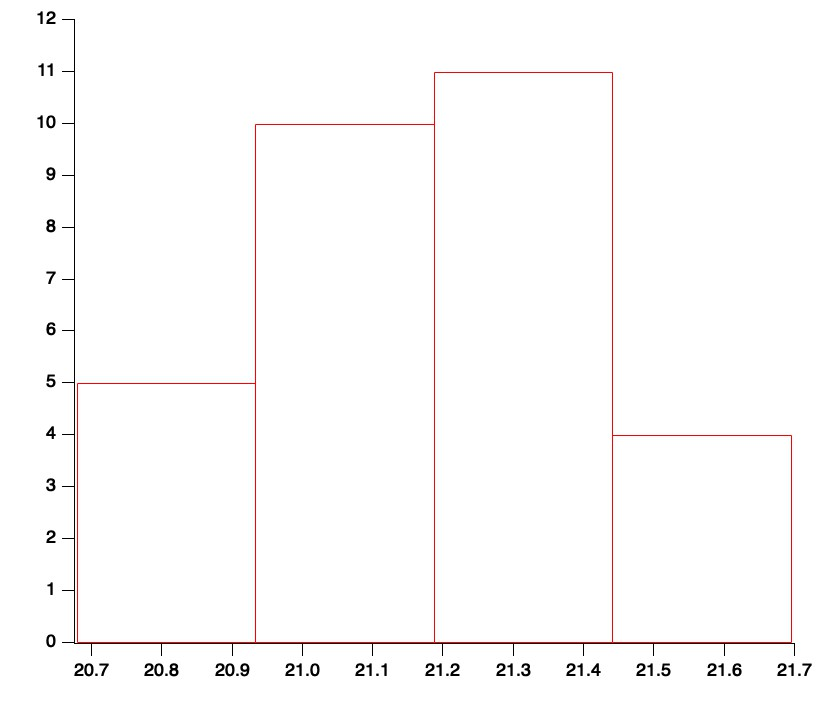
\includegraphics[width=170mm]{Immagini/Histogram Pendolo.jpg}
\caption{\textit{{\footnotesize{L'Istogramma presenta 4 classi, ciascuna con la relativa frequenza (asse $y$) }}}}
\label{Grafico parabolico}
\end{figure}


\bigskip
\addvspace{1.5cm}
La \textit{confidenza} ottenuta, consultando la relativa tabella, è compresa tra il 25\% ed il 50\%, quindi i valori di $10T$ misurati sono compatibili con un campione Gaussiano.

\newpage

\section{Misura di M}
Tramite una bilancia elettronica con sensibilità al decigrammo, sono state pesate le masse campione:

\begin{table}[!htb]
    \centering
        \begin{tabular}{|c|c|}
            \hline
            $N^o$ &Massa M $(kg)$\\
            \hline
            $1$ & $0.0125\pm0.0001$\\
            $2$ & $0.0168\pm0.0001$\\
            $3$ & $0.0222\pm0.0001$\\
            $4$ & $0.0372\pm0.0001$\\
            $5$ & $0.0663\pm0.0001$\\
            \hline
        \end{tabular}
        \label{Tab masse}
        \caption*{Tabella 2: \textit{\footnotesize In Tabella sono riportate le masse campione, in ordine crescente.}}
        \end{table}

    Si considerano le masse come note, quindi con ordine di grandezza dell'errore relativo $<0.1\%$. Per questa ragione, si assumono le masse aventi incertezza nulla.


    
\section{Misura di L}
\label{Misura di L}
Si è poi passati al calcolo della lunghezza del filo al variare della massa appesa. Le misure registrate, tramite un metro a nastro con sensibilità al millimetro, sono le seguenti:

\begin{table}[!htb]
    \centering
        \begin{tabular}{|c|c|c|}
            \hline
            $N^o$ &Massa M $(kg)$&Lunghezza L $(m)$\\
            \hline
            $0$ & $0.0000$         &$1.094\pm0.002$\\
            $1$ & $0.0125\pm0.0001$&$1.095\pm0.002$\\
            $2$ & $0.0168\pm0.0001$&$1.096\pm0.002$\\
            $3$ & $0.0222\pm0.0001$&$1.097\pm0.002$\\
            $4$ & $0.0372\pm0.0001$&$1.099\pm0.002$\\
            $5$ & $0.0663\pm0.0001$&$1.103\pm0.002$\\
           
            \hline
        \end{tabular}
        \label{Tab Lunghezze}
        \caption*{\centering Tabella 3: \textit{\footnotesize In Tabella sono riportate le masse campione e le diverse lunghezze del filo misurate con i rispettivi errori }}
        \end{table}


Come si può osservare dalla Tabella 3, la lunghezza del filo a riposo è $L_0=(1.094\pm0.002)\ m$. Si noti come tutte le lunghezze siano ocnfrontabili, tranne quella corrispondente alla $N^o\ 5$, che vale $L_5=(1.103\pm0.002)\ m$. Questo può essere dovuto al fatto che il filo utilizzato nell'esperimento, si fosse allentato, poichè l'apparato sperimentale è stato usato precedentemente da altri Gruppi. 
Perciò si è deciso di scartare questa misura e non usarla nei calcoli successivi. 

Inoltre si osservi come l'errore relativo $\displaystyle \frac{\Delta L_i}{L_i}$, con $i={0,1,2,3,4,5}$ , è circa dello $0.1\%$.

La lunghezza media del filo $\overline{L}$ è:

\begin{equation*}
\begin{aligned}
  & & \overline{L}=\frac{\sum_{i=0}^{4}L_i}{6-1}=1.096\ m
  &\quad{} 
  \end{aligned}
  \begin{aligned}
  & &\text{dove:\phantom{.......}} \Delta \overline{L}=\sum_{i=0}^{4}=0.010\ m
  &
  \end{aligned}
\end{equation*}
\bigskip

Quindi $\overline{L}=(1.096\pm0.010)\ m$


\section{Indipendenza di T da $\Phi_{max}$}
\label{Indip T da angolo}

Per mostrare per quale intervallo angolare vale l'indipendenza di T dall'ampiezza massima, sono state effettuate 6 misure di dieci periodi, mantenendo la stessa massa $M=(0.0663\pm0.0002)\ kg$ durante tutte le misurazioni, e variando l'angolo, misurato tramite un goniometro posto all'estremità dell'asta rigida che sorregge il pendolo. 
\bigskip

Le misure sono state fatte per angoli di $\Phi_{max1}=(5^o\pm1^o)$, $\Phi_{max2}=(10^o\pm1^o)$, $\Phi_{max3}=(15^o\pm1^o)$, $\Phi_{max4}=(20^o\pm1^o)$, $\Phi_{max5}=(25^o\pm1^o)$, $\Phi_{max6}=(30^o\pm1^o)$.

Importante ricordare che la formula per calcolare il periodo $T$ anche per angoli grandi, arrestandoci al secondo termine dallo sviluppo in serie, è data da:

\begin{equation*}
    T=T' \left(1+\frac{1}{4}\ \sin^2{\left(\frac{\Phi_{max}}{2}\right)}\right)
\end{equation*}

dove il primo termine è dato da:
\begin{equation*}
\begin{aligned}
  & & \displaystyle T'=2\pi\ \sqrt{\frac{\overline{L}}{g_{tab}}}=2.1005\ s
  &\quad{} 
  \end{aligned}
  \begin{aligned}
  & &\text{ e l'errore è:\phantom{.......}} \Delta T'=\left|\frac{d}{d\overline{L}}\left( 2\pi\ \sqrt{\frac{\overline{L}}{g_{tab}}}\right)\right|\cdot\Delta\overline{L}=0.01\ s
  &
  \end{aligned}
\end{equation*}
\bigskip

Quindi $T'$, periodo per angoli piccoli, vale $T'=(2.10\pm 0.01)\ s$, ed è indipendente dall'angolo.


\addvspace{3cm}
I risultati ottenuti a partire dalle misurazioni sono riportati nella seguente tabella:

\begin{table}[ht] 
\centering
\begin{tabular}{|c|c|c|c|c|c|c|} 

 \hline
  &$\Phi_{max1}\ (^o)$ & $\Phi_{max2}\ (^o)$ & $\Phi_{max3}\ (^o)$ & $\Phi_{max4}\ (^o)$ & $\Phi_{max5}\ (^o)$ & $\Phi_{max6}\ (^o)$  \\
    &$(5\pm1)$ & $(10\pm1)$ & $(15\pm1)$ & $(20\pm1)$ & $(25\pm1)$ & $(30\pm1)$  \\
\hline

  $10T$& $21.31\pm 0.05 $&$21.30\pm0.05$&$21.25\pm0.5$&$21.19\pm0.05$ &$21.16\pm0.05$&$21.60\pm 0.05$\\
\hline
 $T$& $2,13\pm 0.05 $&$2.13\pm0.05$&$2.12\pm0.5$&$2.12\pm0.05$ &$2.12\pm0.05$&$2.16\pm 0.05$\\
\hline

\end{tabular}\\
\caption*{\centering Tabella 4:\small{\textit{ } }}
    \label{tab T indip Angolo}
\end{table}


\newpage

Confontando il periodo $T$ misurato, e i valori $T'$ del periodo indipendente dall'angolo, si ottine il seguente grafico:



    \begin{figure}[h!]
\centering
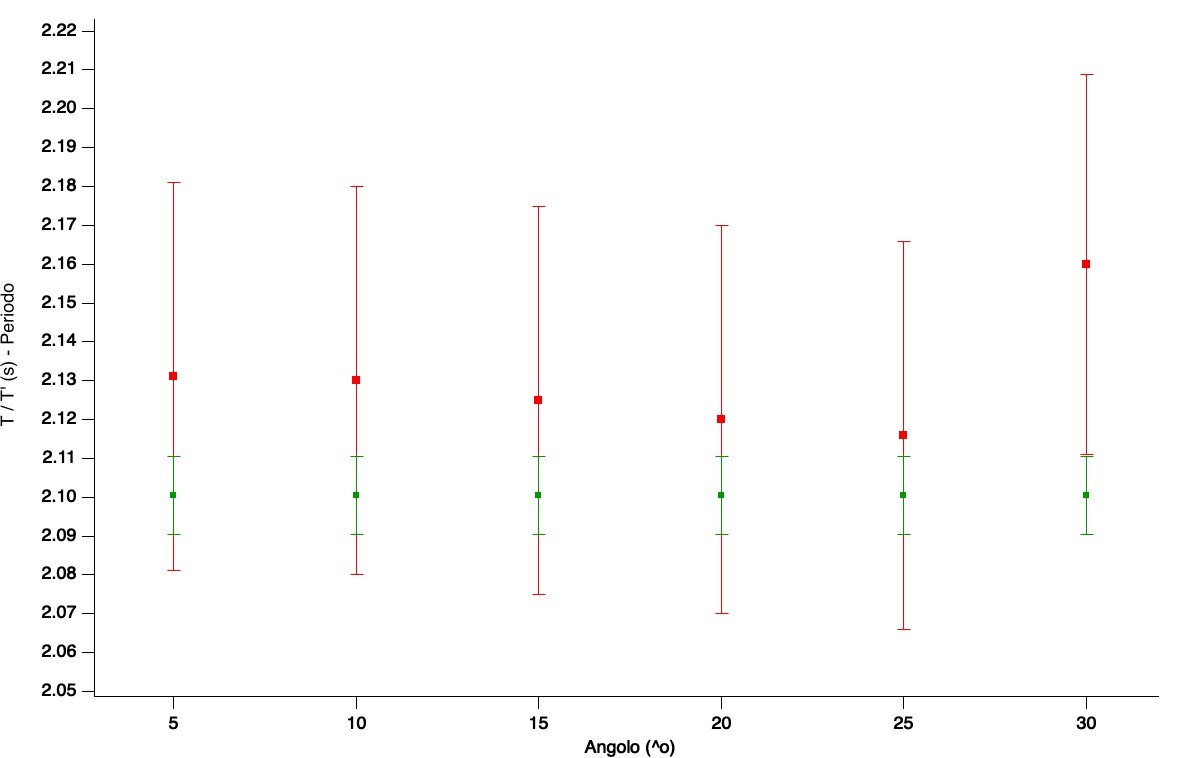
\includegraphics[width=180mm]{Immagini/confrontoTT'.jpg}
\caption{\textit{{\footnotesize{In verde $T'$ misura del periodo indipendente dall'angolo, in rosso $T$ misurato.  }}}}
\label{confrontoTT'}
\end{figure}

Come si può vedere in Figura \ref{confrontoTT'}, fino ad una angolo $\Phi_{max5}=25^o$ il periodo misurato $T$ è compatibile col periodo $T'$ indipendente dall'angolo, mentre per $\Phi_{max6}=30^o$ la misura risulta essere non compatibile. 



\section{Indipendenza di T da M}
\label{Indip T da M}
Si effettuano 5 misurazioni di $10T$, ciascuna con una massa diversa. Si è scelto di far partire l'oscillazione da un angolo fisso pari a $\Phi_{max}=8^o$, così da non avere una dipendenza di $T$ dall'angolo, come mostrato nella Sezione \ref{Indip T da angolo}: \textit{Indipendenza di T da $\Phi_{max}$}, e con una lunghezza del filo costante pari a $\overline{L}=(1.096\pm0.010)\ m$, risultato ottenuto nella Sezione \ref{Misura di L}: \textit{Misura di L}.

I risultti sono riportati in tabella:

\begin{table}[ht] 

\begin{tabular}{|c|c|c|c|c|c|} 

 \hline
  &$M1\ (kg)$ & $M2\ (kg)$ & $M3\ (kg)$ & $M4\ (kg)$ & $M5\ (kg)$   \\
   &\small$(0.0125\pm0.0001)$ & \small$(0.0168\pm0.0001)$ & \small$(0.0222\pm0.0001)$ & \small$(0.0372\pm0.0001)$ & \small$(0.0663\pm0.0001)$ \\
\hline

  $10T$& $21.31\pm 0.05 $&$21.30\pm0.05$&$21.25\pm0.5$&$21.19\pm0.05$ &$21.16\pm0.05$\\
\hline
 $T$& $2,13\pm 0.05 $&$2.13\pm0.05$&$2.12\pm0.5$&$2.12\pm0.05$ &$2.12\pm0.05$\\
\hline

\end{tabular}\\
\caption*{\centering Tabella 5:\small{\textit{ } }}
    \label{tab T indip Angolo}
\end{table}

    \begin{figure}[h!]
\centering
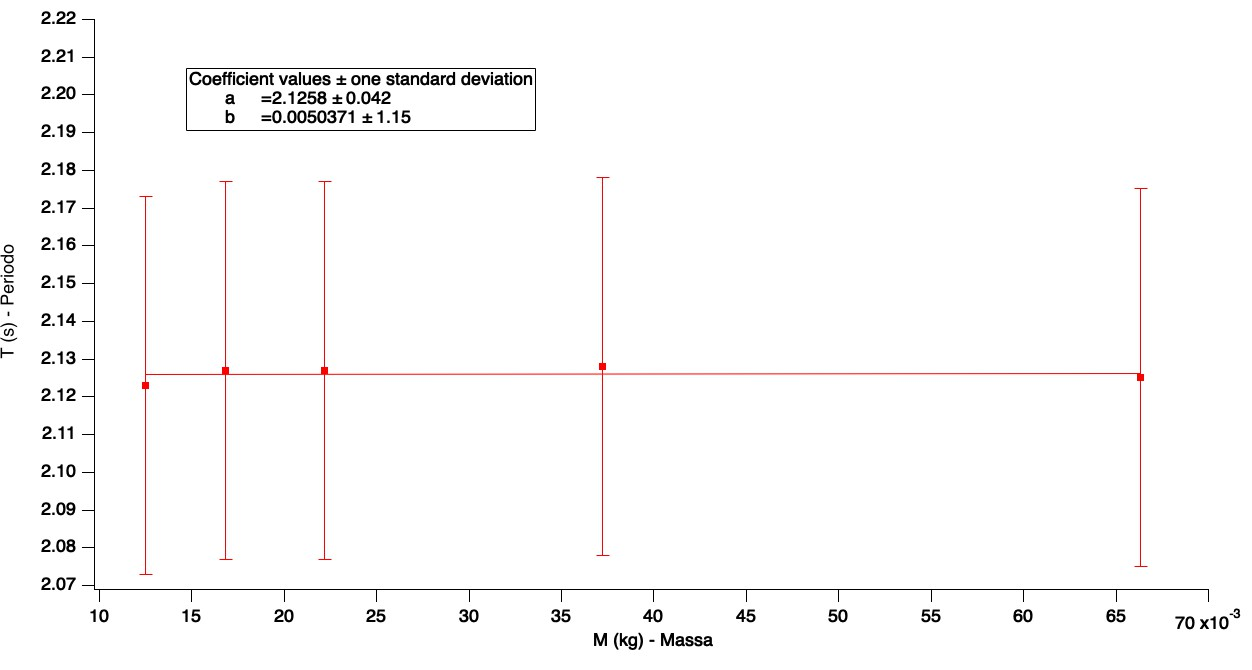
\includegraphics[width=180mm]{Immagini/IndipTdaM.jpg}
\caption{\textit{{\footnotesize{descrizione  }}}}
\label{IndipendenzaTM}
\end{figure}

\newpage
Come si può notare dal Grafico \ref{IndipendenzaTM}, $T$ rimane pressochè costante al variare di $M$ e come conseguenza la retta ottenuta dal \textit{Quick Fit} è orizzontale con pendenza $b=(0.0\pm1.2)$.

Si è quindi verificata l'indipendenza di $T$ da $M$. 
\section{Dipendenza di T ed L}

\section{Misura di g}
\section{Conclusioni}

\end{document}

